
\documentclass{report}

% Ćirilica: kodiranje fonta i jezik (srpski, ćirilica)
\usepackage[T2A]{fontenc}
\usepackage[utf8]{inputenc}
\usepackage[serbianc]{babel}

% Veličina strane i margine
\usepackage[a4paper,top=2cm,bottom=2cm,left=3cm,right=3cm,marginparwidth=1.75cm]{geometry}

% Korisni paketi
\usepackage{amsmath}
\usepackage{graphicx}
\usepackage{float}

\usepackage{subcaption}
\usepackage{enumitem}

\usepackage{booktabs}
\usepackage{tcolorbox}
\tcbuselibrary{breakable}
\usepackage[colorlinks=true, allcolors=blue]{hyperref}

% Цртежи (TikZ)
\usepackage{tikz}
\usetikzlibrary{arrows.meta, calc, decorations.markings, babel}

% TikZ стилови који се понављају на цртежима
\tikzset{
    naboj/.style={circle, draw, thick, minimum size=6mm, inner sep=0pt, font=\small},
    jezgro/.style={circle, draw, thick, fill=gray!15, minimum size=7mm, inner sep=0pt, font=\small},
    elektron/.style={circle, draw, fill=cyan!30, inner sep=0pt, minimum size=5pt},
    supljina/.style={circle, draw, thick, minimum size=5mm, inner sep=0pt, font=\small},
    sredstrelica/.style={postaction={decorate}, decoration={markings, mark=at position 0.55 with {\arrow{Stealth}}}},
    % --- графици наизменичних величина ---
    pomocna/.style={dashed, gray!70, thin},
    mreza/.style={gray!25, very thin},
    kriva/.style={very thick, red!75!black},
    % --- проводник у пресеку: празан, тачка (ка нама), крстић (од нас) ---
    provodnik/.style={circle, draw, thick, fill=white, minimum size=8pt, inner sep=0pt},
    provodnikT/.style={provodnik, path picture={\fill[black] (path picture bounding box.center) circle (1.1pt);}},
    provodnikK/.style={provodnik, path picture={
        \draw (path picture bounding box.south west) -- (path picture bounding box.north east)
              (path picture bounding box.north west) -- (path picture bounding box.south east);}},
    oznaka/.style={fill=white, inner sep=1pt, font=\small},
}

% Оквир за решене примере
\newtcolorbox[auto counter]{primer}{breakable,
    colback=white, colframe=black!55, colbacktitle=black!55, coltitle=white,
    fonttitle=\bfseries\small, title={Пример~\thetcbcounter},
    boxrule=0.5pt, arc=1.5pt, left=6pt, right=6pt, top=3pt, bottom=3pt,
    before skip=8pt, after skip=10pt}

% Оквир за кључне формуле
\newtcolorbox{kljucno}{colback=blue!4, colframe=blue!45!black,
    boxrule=0.5pt, arc=1.5pt, left=8pt, right=8pt, top=4pt, bottom=4pt}

\title{Аутоелектронски системи 2 - Jetronic системи убризгавања}
\author{Саобраћајно техничка школа, Београд, Земун}

\begin{document}
\maketitle

\tableofcontents
\newpage

%==================================================================
% БЕЛЕШКЕ ИЗ СВЕСКЕ (редом по сликама IMG_6501 -- IMG_6508)
%==================================================================

\chapter{Генерализација ОТО мотора} 

За рад моторних возила, већински се користе мотори са унутрашњим сагоревањем од којих је 
једна од могућих реализација, прилично популарна али стара - \textit{ОТО} мотори.

\textit{ОТО} мотори подразумевају четворотактни \textit{(4-тактни)} циклус рада:

\begin{itemize}      % tačke
    \item Први такт - Припрема мешавине + усисавање
    \item Други такт - Сабијање + паљење гаса (експлозија)
    \item Трећи такт - Кретање клипа
    \item Четврти такт - Издувавање
\end{itemize}

За нормално функционисање ОТО-мотора са унутрашњим сагоревањем користимо
се са 2 система, системима убризгавања и системима пањења. Пионир у развијању оба система 
је Немачка фирма \textit{BOSCH}, која је почела са израдом система прва и
која је израдила и усавршила већину стандардне технологије. Ови системи се и дан 
данас усавршавају.
Тренутно ћемо 
споменути само основне системе убризгавања. 

Првобитно у моторима су коришћени карбуратори који су имали константан доток горива. 
Како би се повећало искоришћење, контрола и стабилност мотора уведени су системи убризгавања.

У почетку су били \textbf{механички} или \textbf{хидраулички}(K - KE Jetronic ), а како се унапређивала технологија 
електронских уређаја, тако се и \textbf{електроника} убацивала у ове системе (L - LH - Mono Jetronic) како би корисник
имао већу контролу над мотором. Кроз текст биће више објашњене разлике и зашто је све 
ово битно.

\section{Коефицијент вишка ваздуха}

Бензин у мотор не довлачимо директно, већ прво довучено бензин под притиском претворимо у 
гасно агрегатно станје, односно у гас и онда  га мешамо са ваздухом. Таква комбинација горива
и ваздуха се зове \textbf{смеша}.

Потребно је најпре дефинисати \textbf{коефицијент вишка ваздуха} $\lambda$ (енг. Ламбда). 
Ламбда дефинишемо помоћу следеће формуле: 

\begin{equation}
    \lambda = \frac{\text{доведена количина ваздуха}}{\text{теоријски потребна количина ваздуха}}
\end{equation}

\textbf{Теоријски потребна величина ваздуха} је тзв. стехеометријски однос мешавине ваздуха и бензина.
Тај теоријски потребан однос је избоси приближно 1:14.7. Шта значи то? Како би мотор радио У
оптималном стању, на 1$kg$ је потребно довести 14.7$kg$ ваздуха. Како онда формула која је написана 
горе функционише? 

\begin{itemize}
    \item $\lambda = 1$, направљена је савршен однос смеше
    \item $\lambda < 1$, доведена количина ваздуха је манје од теоријски потребне, смеша је \textbf{богатија горивом}
    \item $\lambda > 1$, доведена количина ваздуха је више од теоријски потребне, смеша је \textbf{сиромашнија горивом}
    \item $\lambda > 1.3$, мотор не може да се упали
\end{itemize}

\section{Подела система убризгавања}

Основна подела система убризгавања је по \textbf{методи регулације} и она чини: 

\begin{itemize}
    \item Хидро-механичка регулација - чисто механичка регулација убризгавања (K - Jetronic).
    \item Механичко електронска регулација - надоградња на механичку регулацију, додата
            електрика ради прецизније регулације (KE - Jetronic).
    \item Електронска регулација - управљање регулацијом помоћу електронске управљачке 
            јединице. Прикупља информације преко сензора и на тај начин одлучује о 
            концентрацији смеше.
\end{itemize}

Сви ови системи регулације важе за убризгавање у више тачака, биће више речи о томе.

Системи убризгавања такође се деле по \textbf{временској} и \textbf{просторној} основи, односно када и 
где убризгавају гориво.

Временска подела: 

\begin{itemize}
    \item Континуално убризгавање - Убризгава се гориво констрантно, под дејство притиска
    \item Симултано убризгавање - Гориво се убризгава понекад, али све бризгаљке одједном. Ради се помоћу електромагнетских бризгаљки.
    \item Групно убризгавање - Гориво се убризгава понекад, али само групе бризгаљки у исто време. Ради се помоћу електромагнетских бризгаљки.
    \item Секвенцијално убризгавање - Гориво се убризгава понекад, али свака бризгаљка појединачно. Ради се помоћу електромагнетских бризгаљки.
\end{itemize}

Просторна подела: 

\begin{itemize}
    \item Убризгавање у више тачака (MPI) - место убризгавања је непосредно пре простора за сагоревање.
        На овај начин засебно за сваки простор за сагоревање добијамо потребну мешавину.
    \item Централно убризгавање (SPI) - убрзгавање се ради преко једне бризгаљке, на место довођења
        горива, тако да се у простор за сагоревање увелико уноси мешавина готива и
        ваздуха, без засебног мешања.
    \item Директно убризгавање место убризгавања је у простору за сагоревање. Бенефит оваквог
        начин убрзигавање је то што у простор за сагоревање уносимо само ваздух, а додајемо гориво накнадно.
        На тај начин, на зидовима мотора се не захвата слој горива и меша је прецизнија. Овакав
        начин мешања могући је само код потпуно електронских система мешања.
\end{itemize}

\begin{figure}[H]
    \centering
    \begin{minipage}{0.32\textwidth}
        \centering
        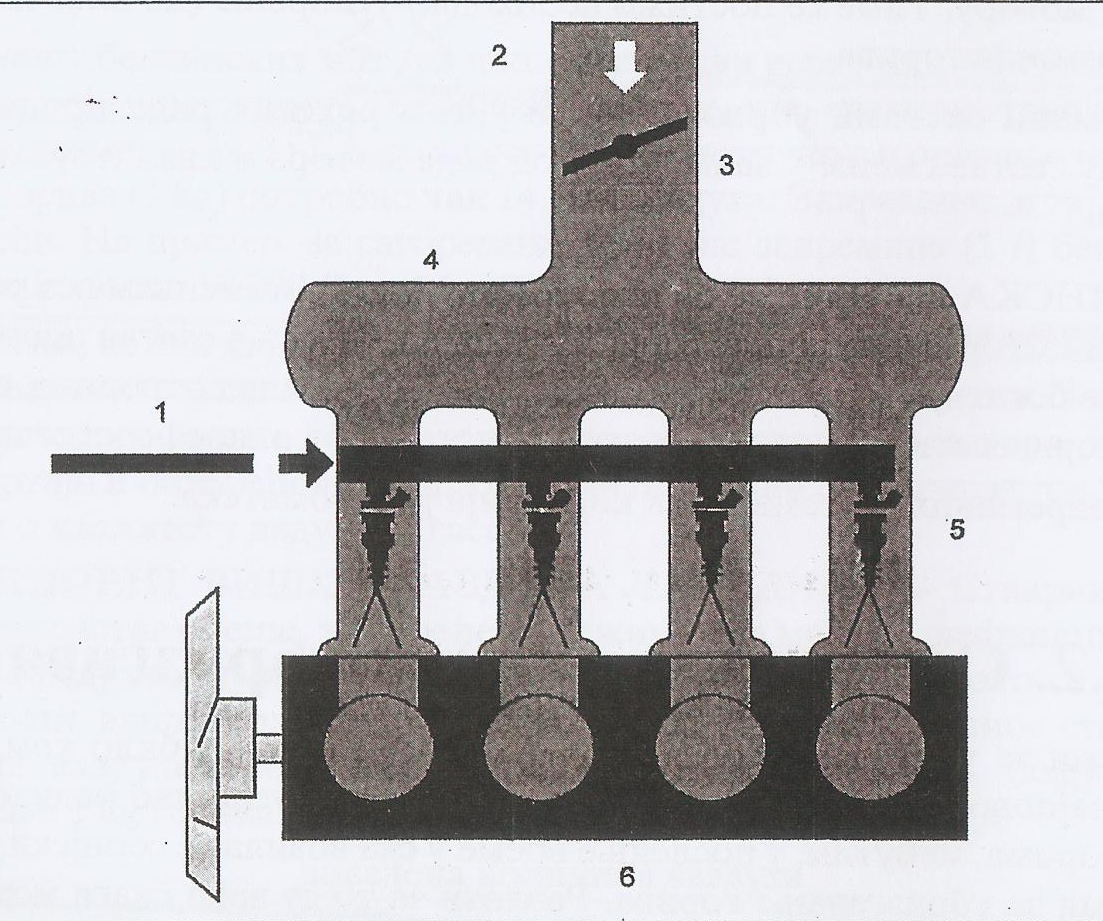
\includegraphics[width=\linewidth]{slike/engineE.png}
        \caption{Убризгавање у више тачака}
        \label{fig:slika1}
    \end{minipage}
    \hfill
    \begin{minipage}{0.32\textwidth}
        \centering
        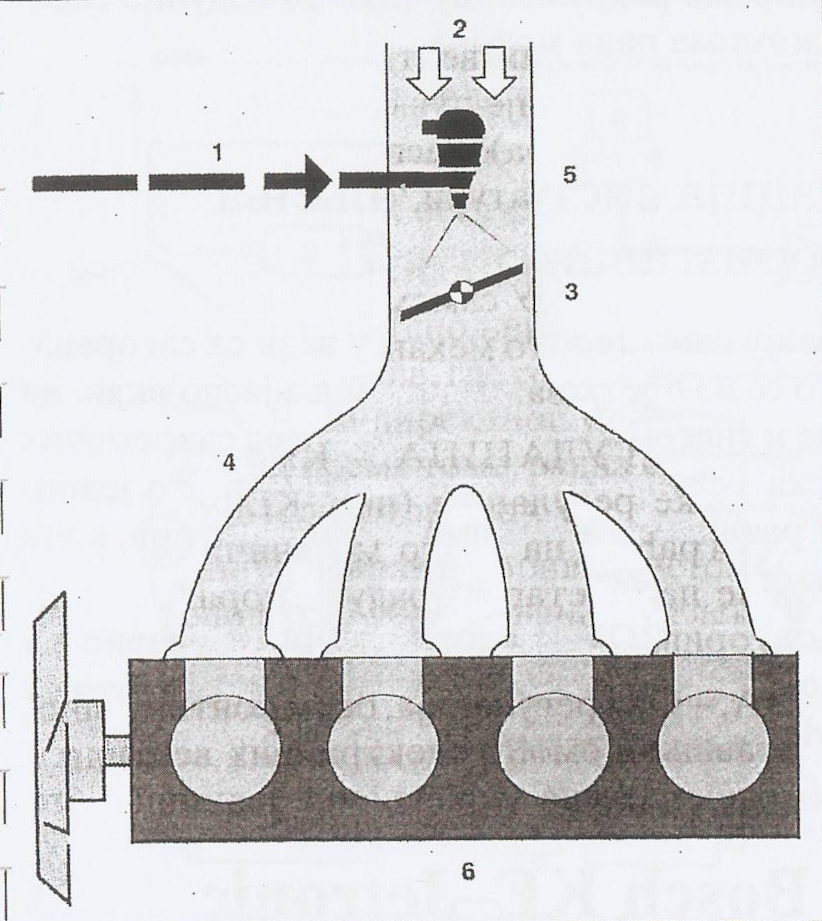
\includegraphics[width=\linewidth]{slike/engine2E.png}
        \caption{Централно убризгавање}
        \label{fig:slika2}
    \end{minipage}
    \hfill
    \begin{minipage}{0.32\textwidth}
        \centering
        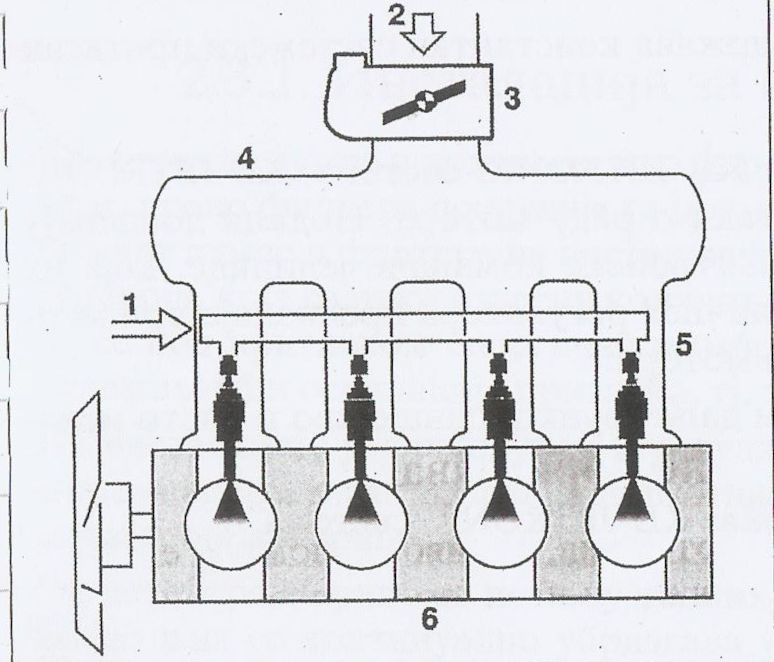
\includegraphics[width=\linewidth]{slike/engine2E2.png}
        \caption{Фиректно убризгавање}
        \label{fig:slika3}
    \end{minipage}
\end{figure}


\section{Контрола рада мотора прилагођавањем смеше}

Како се мења стање мотора кроз циклус рада, тако је потребно прилагођавати смешу у мотору
како би што оптимизованје радио у задатим условима, ипак је то могућност коју нам 
системи убризгавања пружају.

Основна стања у којима мотор може да се нађе, и начин на који се прилагођава смеша,
задати су следећом поделом.

\textbf{Хладан старт} - $\lambda < 1$, због хладног мотора потребно је довести више
горива како би се брже загрејао мотор и довео у оптимално температурнос стање.

\textbf{Загревање} - $\lambda < 1$, одмах после паљења мотор је још хладан, па су потребни
богатија смеша и мало већи број обртаја како би мотор радио сигурно и мирно док се не загреје.

\textbf{Празан ход} - $\lambda < 1$, при најмањем броју обртаја већина мотора тешко ради
стабилно са теоријском смешом, па се смеша мора обогатити. Новији мотори са електронским
паљењем и убризгавањем раде мирно и са $\lambda \approx 1$.

\textbf{Делимично оптерећење} - $\lambda \geq 1$, најчешћи и најдужи режим рада током вожње,
па је циљ што мања потрошња горива и поштовање прописа о издувним гасовима.

\textbf{Пуно оптерећење} - $\lambda < 1$, при потпуно отвореном лептиру
мотор развија највећу снагу, за шта је потребна богатија смеша. Овај режим кратко траје,
па лошији састав издувних гасова не загађује знатно околину.

\textbf{Убрзање} - $\lambda < 1$, наглим отварањем лептира расте притисак у усисној цеви,
гориво слабије испарава и део се хвата на зидовима као танак филм, па се смеша осиромашује.
Зато се додаје више горива, како би мотор добро реаговао и убрзавао без застоја.

\textbf{Кочење мотором} - $\lambda > 1$, одузимањем гаса затвара се лептир и смањује довод
горива, чиме се постиже успорење и уштеда горива. Савремени системи и у овом режиму
прецизно регулишу састав смеше.

\textbf{Висинска корекција} - $\lambda \approx 1$, на већим висинама ваздух је ређи, мотор
усисава мању масу ваздуха и смеша постаје богатија (без корекције $\lambda < 1$). Да не би
расла потрошња, количина горива се коригује према атмосферском притиску, а код савремених
система то се ради аутоматски.

\chapter{KE-Jetronic систем убризгавања} 

Слика система и његових компоненти дата је испод. Како су се модели система убризгавања мењали, само неке од компоеннти 
су се мењале, већином су остале исте. Зато се анализа система ради од најстарије, па до најновије.

\begin{figure}[H]
    \centering
    \includegraphics[width=0.7\textwidth]{slike/KEe.png}
    \caption{Основна шема KE Jetronic система убризгавања}
    \label{fig:primer}
\end{figure}

\begin{enumerate}
    \item[1.] Резервоар за гориво - место са бензином
    \item[2.] Електрична пумпа за гориво - усисавање бензина
    \item[3.] Хидраулична пригушница за гориво - регулација константног притиска
    \item[4.] Филтер за гориво 
    \item[5.] Регулатор системског притиска - одржавање притиска
    \item[6.] Бризгаљка 
    \item[7.] Усисни колектор 
    \item[8.] Бризгаљка за хладан старт
    \item[9.] Дозатор - Комора за дозирање бризгаљки
    \item[10.] Мерач протока ваздуха (протокомер)
    \item[11.] Електро-хидраулични регулатор (актуатор)
    \item[12.] ЛАМБДА сонда - сензор мешавине
    \item[13.] Временски термо-прекидач 
    \item[14.] Сензор температуре мотора
    \item[15.] Разводник паљења 
    \item[16.] Регулатор празног хода
    \item[17.] Потенциометар пригушног лептира
    \item[18.] Електронска управљачка јединица
    \item[19.] Контакт-кључ
    \item[20.] Акумулатор
\end{enumerate}

%==================================================================
% КОМПОНЕНТЕ KE-JETRONIC СИСТЕМА
%==================================================================

\section{Електрична пумпа за гориво}

Пумпа усисава гориво из резервоара и потискује га под притиском од око 5 бари.
Покреће је електромотор једносмерне струје и гориво гура даље ка разводнику горива.

Ротор пумпе је обртна плоча са жлебовима у којима се налазе покретни ваљчићи.
Плоча је мало са стране тако да је простор између ње и кућишта велики на
усисној страни, а мали на потисној. Када се плоча окреће, центрифугална сила
избацује ваљчиће ка зиду кућишта. Они захватају гориво на ширем, усисном делу и
потискују га ка ужем, потисном делу, где му расте притисак.

\begin{figure}[H]
    \centering
    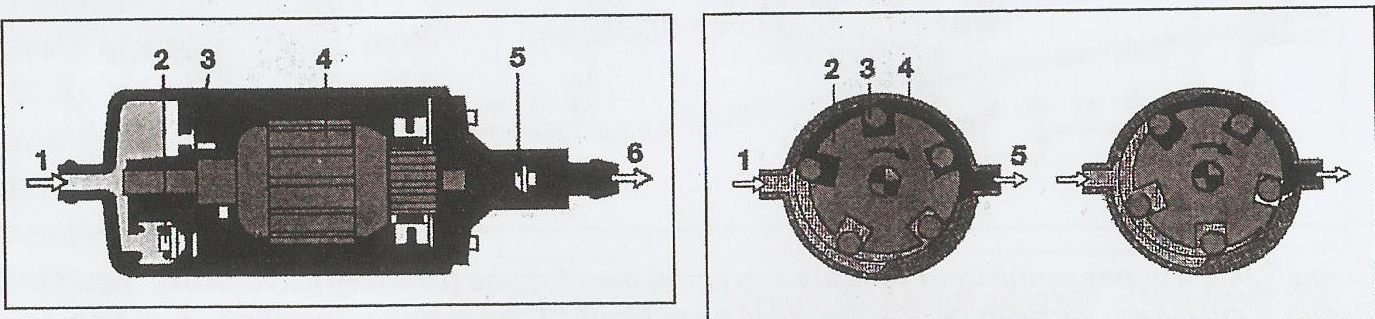
\includegraphics[width=0.7\textwidth]{slike/KEe1.png}
    \caption{Електрична пумпа за гориво}
    \label{fig:primer}
\end{figure}

Пумпа се напаја преко контакт-кључа и заштитног релеја. Ако мотор не ради, а
контакт је укључен (нпр. после саобраћајне незгоде), реле искључује пумпу.

\subsection{Хидраулична пригушница (шпајхер)}

Пригушница после гашења мотора и пумпе још неко време одржава притисак горива у
систему, што олакшава поновно паљење загрејаног мотора. Док пумпа ради,
пригушује буку и ублажава падове притиска.

\begin{figure}[H]
    \centering
    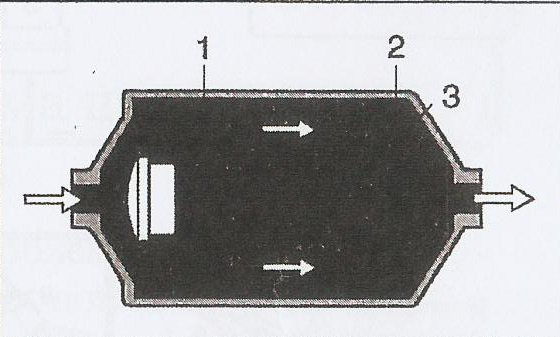
\includegraphics[width=0.4\textwidth]{slike/KEe2.png}
    \caption{Хидраулична пригушница}
    \label{fig:primer}
\end{figure}

Еластична мембрана дели пригушницу на две коморе. У једној је гориво под
притиском, а у другој ваздух (на атмосферском притиску) и спирална опруга. Док
пумпа ради, гориво пуни своју комору и потискује мембрану и опругу до
одбојника. Када се пумпа угаси, опруга гура мембрану назад, гориво се из коморе
враћа у инсталацију и притисак остаје одржан.

\subsection{Филтер за гориво}

Филтер задржава нечистоће из горива. Састоји се од папирног улошка са порама од
око 10 микрона и сита које придржава перфорирана плоча, смештених у метално
кућиште.

Уграђује се у главни вод, после хидрауличне пригушнице. Стрелица на кућишту
показује смер протока горива и мора се поштовати при замени. Трајање улошка
зависи од квалитета и чистоће горива.

\subsection{Регулатор системског притиска}

Регулатор одржава сталан притисак горива у систему. Код KE-Jetronic-а
хидраулички притисак на клипу разводника једнак је системском притиску, па свака
његова промена мења састав смеше. Зато тај притисак мора бити тачно одржаван.

\begin{figure}[H]
    \centering
    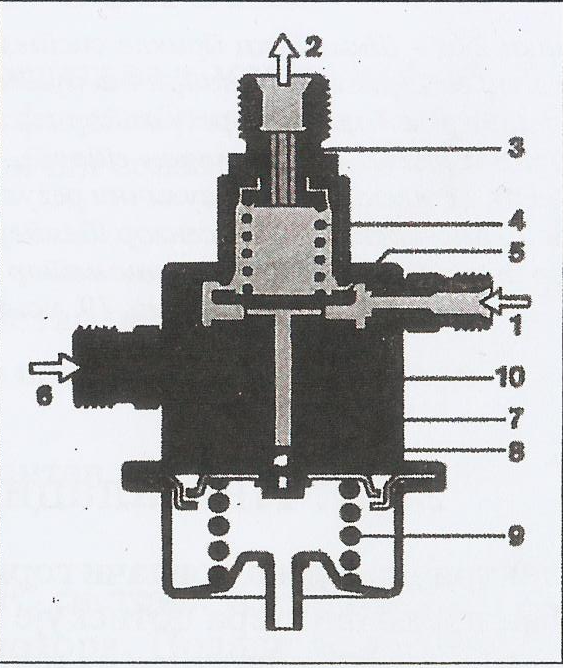
\includegraphics[width=0.4\textwidth]{slike/KEe22.png}
    \caption{Регулатор системског притиска}
    \label{fig:primer}
\end{figure}

[6. ] Довод горива, [2. ] Одвод горива, [1. ] Повратни вод од разводника

Када пумпа проради, притисак горива спушта мембрану, која сабија регулациону
опругу. Заједно са мембраном спушта се и тело вентила и отвара повратни ток ка
резервоару. Вишак горива из разводника тако се враћа у резервоар, а мембрана,
уз потисак опруге, одржава притисак сталним.

Када се мотор угаси, пумпа стаје и притисак опада. Вентил затвара прелив, опруга
подиже мембрану, а тело вентила затвара и повратак горива у резервоар. Притисак
падне толико да се затворе бризгаљке, а затим га у систему одржава хидраулична
пригушница.

\subsection{Бризгаљке (дизне)}

Бризгаљке распршују гориво у усисну цев, испред усисног вентила. Оне гориво не
дозирају, већ га само распршују, а количину одређује разводник.

Бризгаљка се сама отвара када притисак горива пређе одређену вредност (нпр.
3,5 бари). Притисак помери иглицу и отвори млазницу, после чега притисак мало
опадне и иглица се поново затвори, па се процес понавља. Иглица тако вибрира
великом учестаношћу, што гориво добро распршује, нарочито при малим количинама.

Када се мотор угаси, бризгаљке се затварају чим притисак падне испод притиска
отварања, тако да у систему остаје бар око 2,5 бари. Причвршћују се посебним
држачима који их штите од топлоте мотора.

\begin{figure}[H]
    \centering
    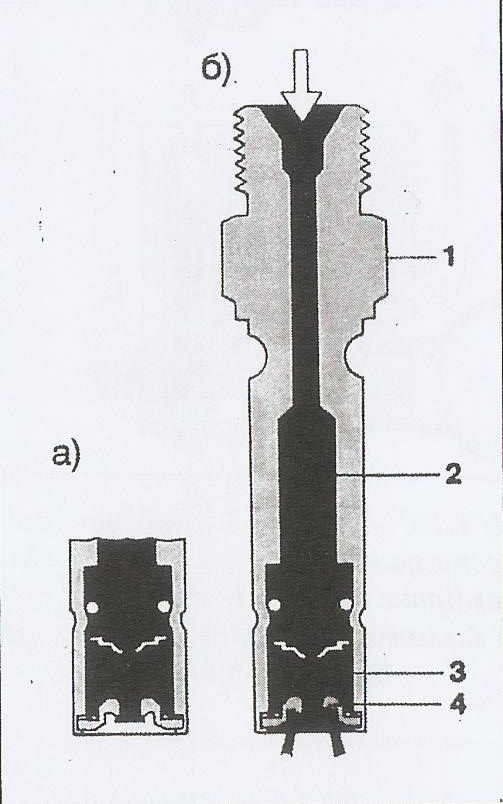
\includegraphics[width=0.4\textwidth]{slike/KEe31.png}
    \caption{Бризгаљке}
    \label{fig:primer}
\end{figure}

\subsection{Мерач протока ваздуха (протокомер)}

Основна величина према којој се дозира гориво је количина усисаног ваздуха, па
се она стално мери. Сав усисни ваздух пролази кроз протокомер, који се налази
испред пригушног лептира.

У левкастој цеви налази се мерна плоча која лебди у струји ваздуха. Што је
проток већи, ваздух јаче подиже плочу ка ширем делу левка. Померај плоче је
сразмеран протоку ваздуха и преко полуге се преноси на регулациони клип
разводника горива. Тежину плоче и полуге уравнотежује противтег, а лисната
опруга држи плочу у нултом положају када мотор не ради.

\begin{figure}[H]
    \centering
    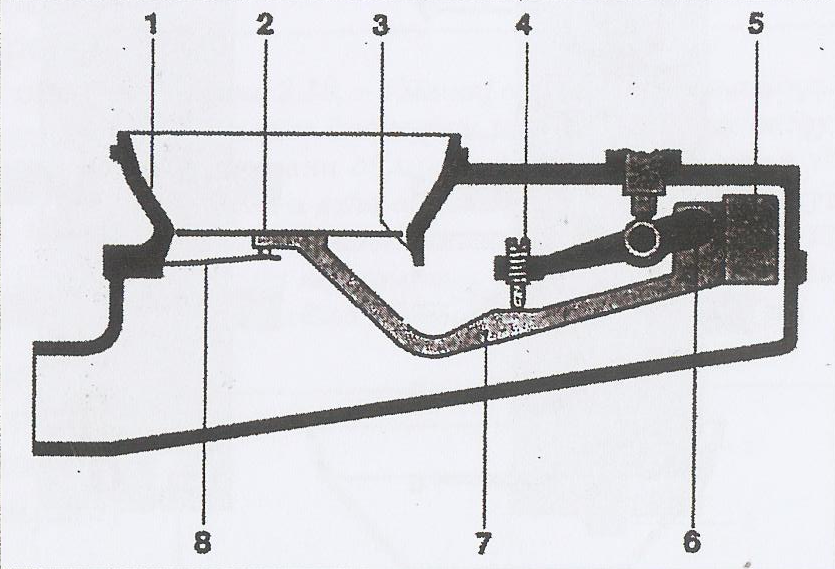
\includegraphics[width=0.4\textwidth]{slike/KEe3.png}
    \caption{Протокомер}
    \label{fig:primer}
\end{figure}

Ако дође до повратног удара из усисне цеви (нпр. због погрешног паљења), плоча
пролети наниже и отвори проширени пресек за растерећење, па се осетљиви делови
протокомера не оштете.

\subsection{Дозатор}

Компонента која сачињава дозатор је \textbf{разводник количине горива}

Разводник дозира гориво и разводи га до бризгаљки, према количини усисаног
ваздуха. Померај мерне плоче преноси се на регулациони клип. Што се клип више
подигне, већи је отвор регулационих прореза (по један за сваки цилиндар) и кроз
њих протиче више горива. Веза између отклона мерне плоче и отвора прореза је
линеарна.

Са друге стране на клип делује притисак горива, који уравнотежује силу ваздуха
на мерну плочу, па клип тачно прати кретање плоче. Зато системски притисак мора
бити тачно регулисан, јер свака његова промена директно мења $\lambda$. Када се
мотор угаси, клип се спусти на заптивни прстен и спречава одлив горива.

\begin{figure}[H]
    \centering
    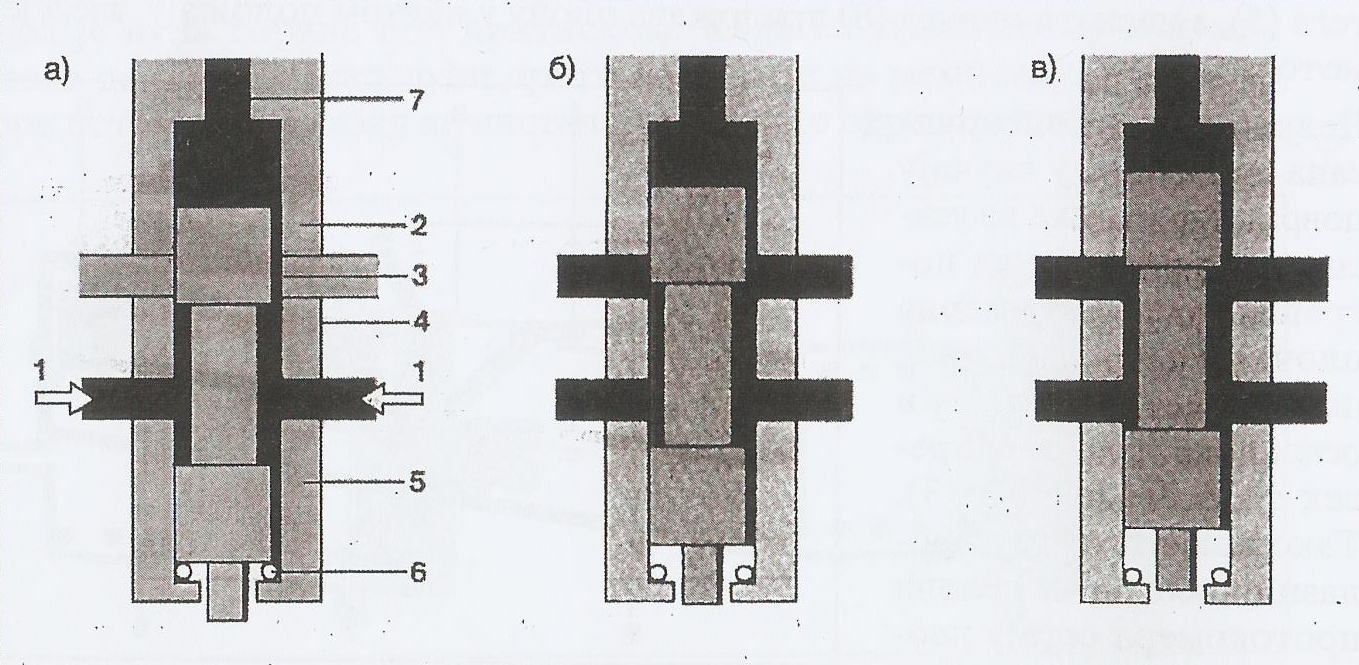
\includegraphics[width=0.7\textwidth]{slike/KEe4.png}
    \caption{Разводник количине горива}
    \label{fig:primer}
\end{figure}

Додатна компонента која сачињава дозатор је \textbf{вентил диференцијалног притиска}
која се у дозатору налази са горње стране.

Ови вентили (по један за сваки цилиндар) одржавају сталну разлику притиска, од
око 0,2 бари, на регулационим прорезима разводника. Пошто је карактеристика
протокомера линеарна, количина горива ће се мењати у истој сразмери као
количина ваздуха само ако је тај пад притиска сталан.

\begin{figure}[H]
    \centering
    \begin{subfigure}{0.4\textwidth}
        \centering
        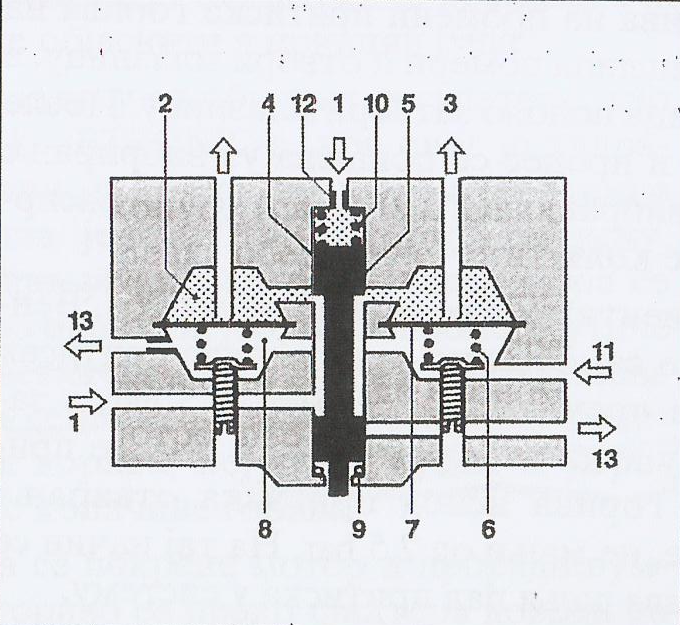
\includegraphics[width=\linewidth]{slike/KEe41.png}
        \caption{}
        \label{fig:deo1}
    \end{subfigure}
    \hfill
    \begin{subfigure}{0.4\textwidth}
        \centering
        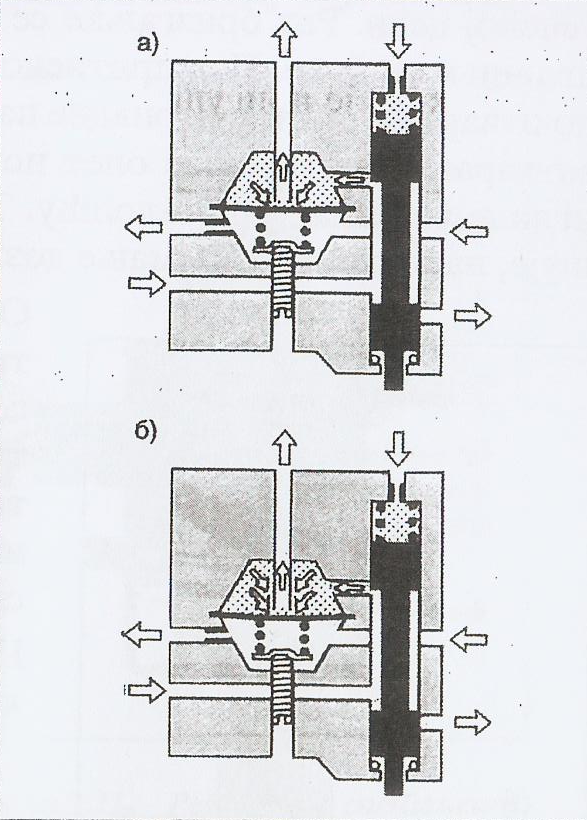
\includegraphics[width=\linewidth]{slike/KEe42.png}
        \caption{}
        \label{fig:deo2}
    \end{subfigure}
    \caption{Вентил диференцијалног притиска}
    \label{fig:obe}
\end{figure}

Челична мембрана дели вентил на горњу и доњу комору. У доње коморе стиже гориво
од актуатора, а горње су повезане са регулационим прорезима и из њих гориво иде
ка бризгаљкама. Када је проток горива мањи, мембрана се мање извије и вентил се
мање отвори, а када је већи, више. Тако се при свакој количини горива на
прорезима одржава исти пад притиска.

Е сада долазимо на питање, како се у дозатору \textbf{формира смеша}.

Смеша се формира у усисној грани и у цилиндру. Гориво се убризгава непрекидно
и нагомилава испред усисног вентила. Када се вентил отвори, ваздух понесе
испарено гориво, а турбуленција у цилиндру га меша у запаљиву смешу.

\begin{figure}[H]
    \centering
    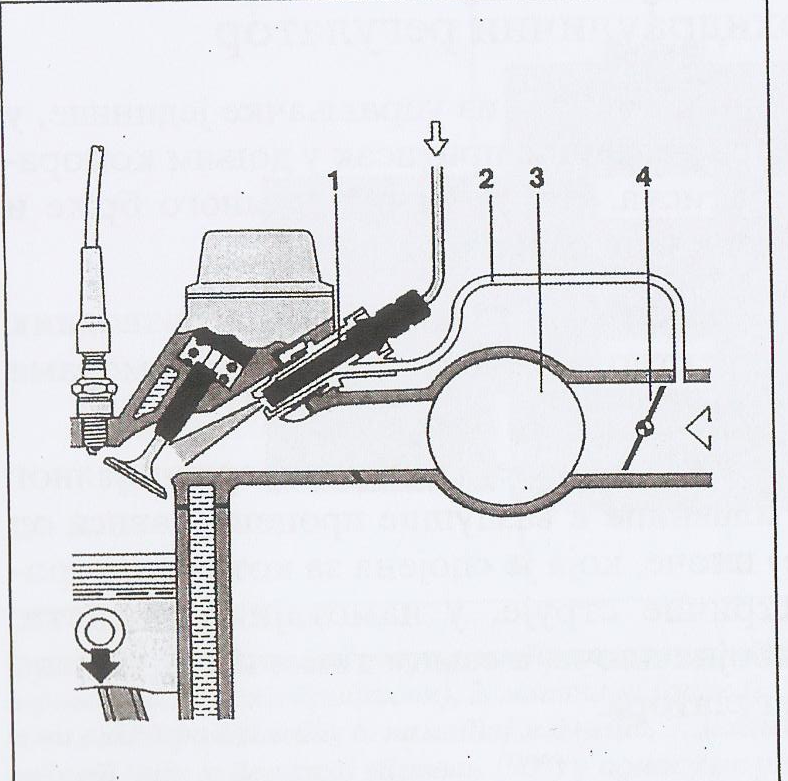
\includegraphics[width=0.4\textwidth]{slike/KE5e.png}
    \caption{Формирање смеше}
    \label{fig:primer}
\end{figure}

За боље распршивање користе се бризгаљке са доводом додатног ваздуха. Мала
количина ваздуха пролази кроз саму бризгаљку и на излазу из млазнице носи
гориво у цилиндар. Ваздух струји због разлике притисака испред и иза пригушног
лептира, па је ефекат највећи при малом оптерећењу и у празном ходу, када је
лептир притворен.

\subsection{Електрохидраулични регулатор (актуатор)}

Актуатор, према електричним импулсима из управљачке јединице, мења притисак у
доњим коморама вентила диференцијалног притиска. Тако се убризгана количина
горива коригује много брже и прецизније, у зависности од режима рада мотора.

Уграђен је на дозер. Гориво под системским притиском пролази кроз
млазницу, испред које је одбојна плоча [11. ] спојена са котвом електромагнета. Струја
кроз намотаје електромагнета, заједно са сталним магнетом, ствара обртни момент
на котви који је сразмеран јачини струје. Тиме се подешава положај одбојне
плоче, а самим тим и пад притиска горива између улаза и излаза регулатора.
Промена притиска у доњим коморама преноси се на горње и мења количину горива
према бризгаљкама.

\begin{figure}[H]
    \centering
    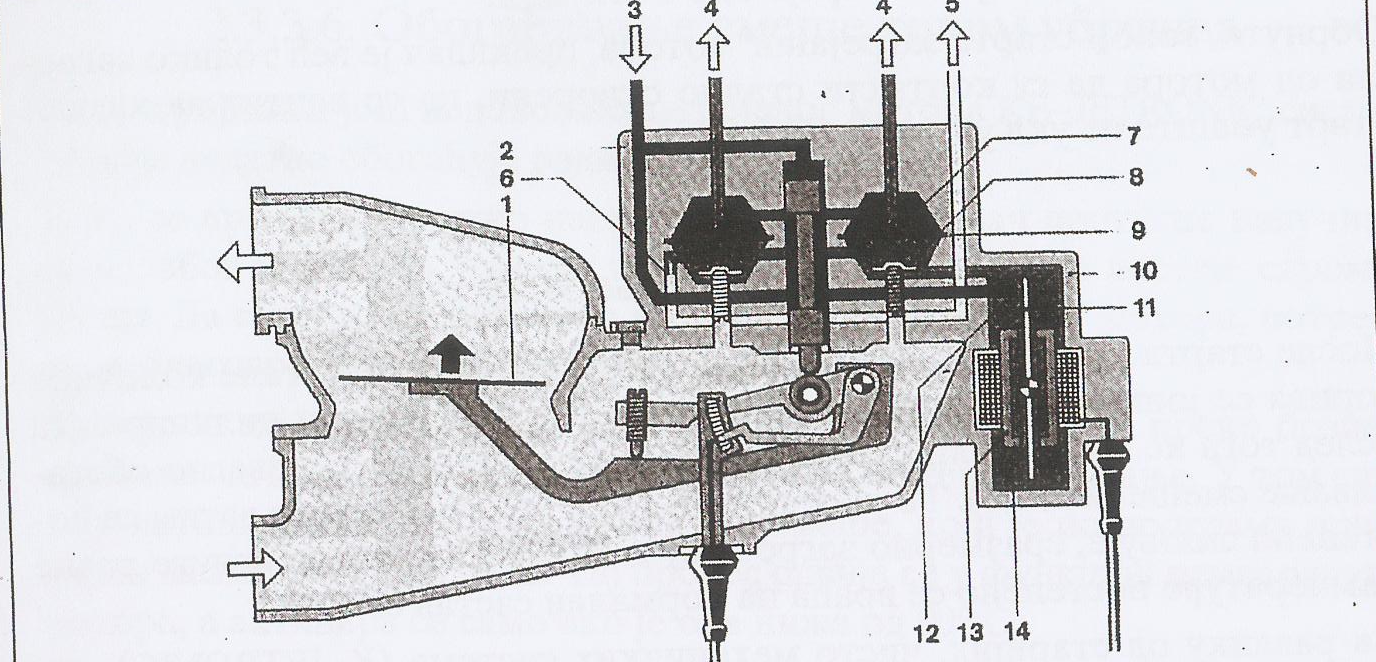
\includegraphics[width=0.4\textwidth]{slike/KE6e.png}
    \caption{Формирање смеше}
    \label{fig:primer}
\end{figure}

Због мале инерције покретних делова регулатор реагује веома брзо. Ако се
промени смер струје, плоча се одмакне од млазнице и бризгаљке потпуно престају
да добијају гориво, што се користи код кочења мотором и ограничења броја
обртаја. Ако нестане струје (квар), регулатор је механички подешен да одржава
$\lambda = 1$, па се возилом може доћи до сервиса.

%==================================================================
% РЕЖИМИ РАДА МОТОРА
%==================================================================

\section{Режими рада КЕ мотора}

Основну количину горива одређује протокомер. Управљачка јединица је, преко
актуатора, додатно коригује према режиму рада мотора и сигналима са сензора.

\subsection{Хладан старт}

При старту хладног мотора велики део горива остаје течан на хладним зидовима
усисне цеви и цилиндра. Смеша постаје сиромашна, често испод границе
запаљивости ($\lambda > 1{,}3$). Зато се додатно гориво убризгава кроз
бризгаљку за хладан старт, коју укључује временски термопрекидач.

\textbf{Бризгаљка за хладан старт} налази се у усисном колектору, иза
пригушног лептира, па гориво подједнако стиже до свих цилиндара. Отвара је
електромагнет. У мировању опруга држи језгро на седишту и бризгаљка је
затворена. Када се електромагнет укључи, језгро се подигне и гориво потекне
ка млазници, где добија вртложно кретање и добро се распршује.

\textbf{Временски термопрекидач} ограничава рад бризгаљке по времену и по
температури. У њему је биметални контакт, који греје електрична спирала и
топлота мотора. Прекидач је у облику сонде, увијен у блок мотора, са врхом у
расхладној течности. Спирала после 8-15 секунди искључује бризгаљку, да се мотор не
би гушио од пребогате смеше. Код загрејаног мотора (изнад око $35^\circ$C)
контакти су стално отворени и бризгаљка се уопште не укључује.

\subsection{Загревање мотора}

После старта део горива се и даље кондензује на хладним зидовима. Да не би
било прекида у паљењу, смеша мора бити богатија ($\lambda < 1$). Обогаћивање
је највеће на почетку и смањује се како се мотор загрева, док на радној
температури смеша не постане нормална.

Код KE-Jetronic-а ово ради управљачка јединица, преко актуатора, а не
механички регулатор као код K-Jetronic-а. Почетно обогаћивање зависи од
температуре мотора, а затим опада приближно линеарно са временом. На пример,
при старту на $+20^\circ$C почетна вредност траје око 5~s, а затим се за око
20~s смеша враћа на нормалу.

\textbf{Сензор температуре мотора} је температурно зависни отпорник у облику сонде, увијен у
блок мотора, са врхом у расхладној течности. Његов отпор опада са порастом
температуре, па управљачка јединица из отпора зна колико је мотор загрејан.

\subsection{Обогаћивање смеше током убрзања}

Када се пригушни лептир нагло отвори(дода гас на педали), нагло порасте количина ваздуха и смеша
накратко постаје сиромашна. Да би мотор добро реаговао на гас на педали, управљачка
јединица благовремено повећава количину горива преко актуатора. Ово
обогаћивање се укључује само ако је мотор хладнији од $80^\circ$C.

Захтев за убрзање управљачка јединица препознаје по брзини промене сигнала са
потенциометра мерне плоче. Сигнал је највећи при поласку из празног хода, а
опада са порастом снаге мотора.

\textbf{Потенциометар мерне плоче} уграђен је у протокомер. Клизачи, спојени
са осовином мерне плоче, клизе по отпорној плочици, па напон потенциометра
зависи од положаја мерне плоче. Клизачи могу да изађу и ван мерног подручја,
па се потенциометар не оштети при повратном удару из усисне цеви.

\subsection{Обогаћивање смеше при пуном оптерећењу}

При делимичном оптерећењу смеша се подешава за најмању потрошњу и најмању
емисију штетних гасова. При пуном оптерећењу смеша се обогаћује, како би
мотор давао највећи обртни момент на целом подручју обртаја.

Управљачка јединица добија сигнал оптерећења од прекидача пригушног лептира,
а сигнал броја обртаја од система паљења. На основу њих коригује количину
горива преко актуатора.

\textbf{Прекидач пригушног лептира} постављен је на кућиште лептира и окреће
се заједно са осовином лептира. Има два контакта: један се затвара у
положају празног хода, а други при пуном оптерећењу.

\subsection{Празан ход хладног мотора}

Хладан мотор има веће унутрашње губитке (трење), па тешко ради у празном
ходу. Зато му се повећава број обртаја, што помаже и бржем загревању.
Додатни ваздух доводи се заобилазним водом (bypass) око пригушног лептира.
Протокомер региструје тај ваздух, па се у истој сразмери повећава и количина
горива.

\textbf{Биметални вентил} регулише проток кроз заобилазни вод. Када је мотор
хладан, отвор вентила је највећи. Како се биметал загрева, електричним
грејачем и топлотом мотора, отвор се смањује, док се код загрејаног мотора
потпуно не затвори.

\subsection{Празан ход}

Биметални вентил не прати стварни број обртаја, већ додаје ваздух само према
температури. Зато се са старењем мотора број обртаја у празном ходу
непотребно повећава, а са њим и потрошња.

\textbf{Регулатор празног хода} то решава. Током целог рада одржава стабилан и
што мањи број обртаја, без обзира на оптерећење и старење мотора. Налази се
у заобилазном воду. Управљачка јединица упоређује стварни број обртаја са
програмираним (који зависи од температуре мотора). Ако се разликују,
регулатор отвара или притвара заобилазни вод док се не постигне жељена
вредност. Регулатор ради као обртни магнет: окреће плочу за око $60^\circ$ и
тако отвара или затвара канал.

\begin{figure}[H]
    \centering
    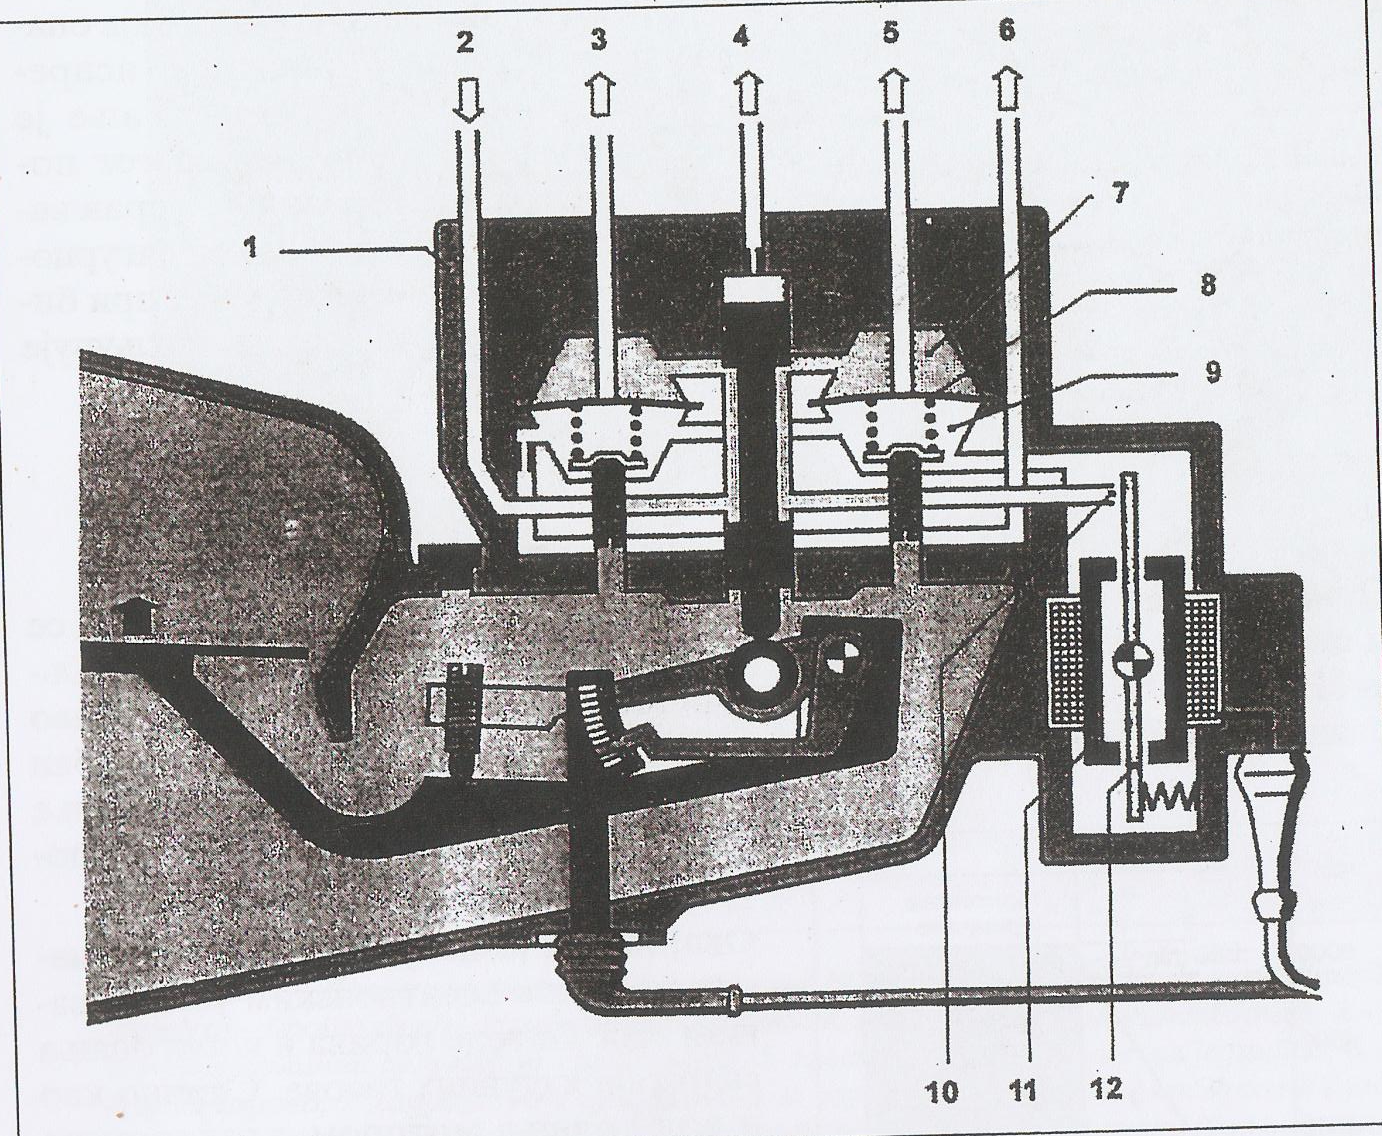
\includegraphics[width=0.4\textwidth]{slike/KEe7.png}
    \caption{Регулатор празног хода}
    \label{fig:primer}
\end{figure}

%==================================================================
% ФУНКЦИЈЕ ОГРАНИЧЕЊА
%==================================================================

\section{Управљаче функције}

Помоћу актуатора, управљачка јединица може да смањи или потпуно прекине
убризгавање горива у одређеним условима. Тиме се штеди гориво, мотор се
штити од превеликог броја обртаја и смањују се штетни издувни гасови.

\subsection{Кочење мотором}

Када возач пусти гас, а возило и даље иде (низбрдица, градска вожња), гориво
није потребно, па се убризгавање прекида. Тиме се штеди гориво и смањују
штетни гасови.

Управљачка јединица препознаје кочење мотором када је пригушни лептир
затворен (сигнал са прекидача лептира), а број обртаја већи од празног хода
(сигнал од система паљења). Тада мења смер струје у актуатору. Притисак у
доњим коморама вентила диференцијалног притиска порасте, мембране затворе
одводе ка бризгаљкама и убризгавање престаје.

\begin{figure}[H]
    \centering
    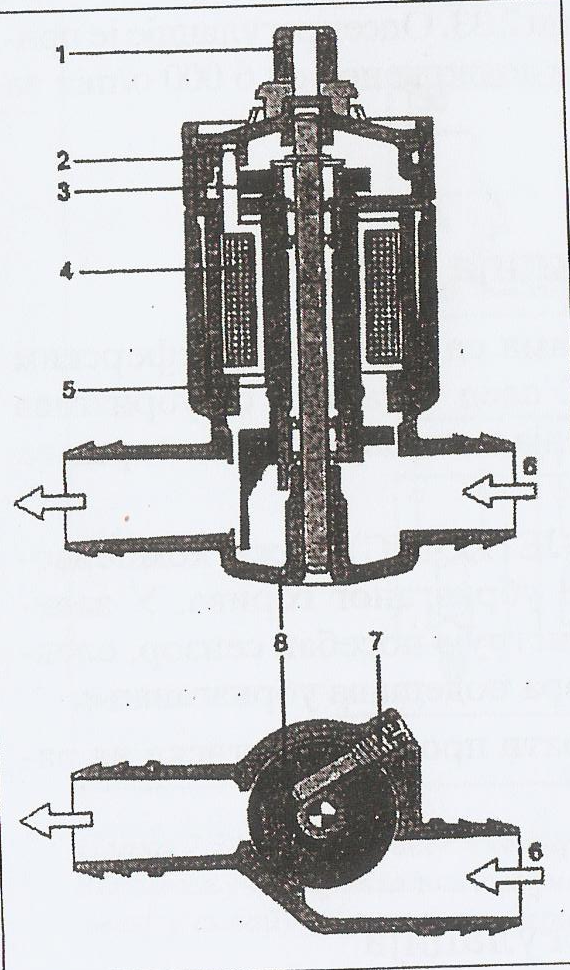
\includegraphics[width=0.4\textwidth]{slike/KEe72.png}
    \caption{Затварање актуатора}
    \label{fig:primer}
\end{figure}

Праг искључења зависи од температуре мотора. Код загрејаног мотора гориво се
искључује већ при мањем броју обртаја, а код хладног тек при већем, да се
мотор не би гасио. Између прага искључења и прага поновног укључења постоји
размак, да се напајање не би стално укључивало и искључивало.

\subsection{Ограничење броја обртаја}

Да би се мотор заштитио, управљачка јединица ограничава највећи број обртаја
прекидањем довода горива бризгаљкама. Раније се то радило преко система
паљења, али прекид горива штеди гориво и смањује штетне гасове.

Када мотор достигне највећи дозвољени број обртаја, управљачка јединица мења
смер струје у актуатору и прекида довод горива. Затим наизменично искључује
и укључује напајање, па се број обртаја одржава у опсегу од око $\pm 80$~o/min
око максималног (нпр. 6\,000~o/min).

\subsection{Висинска корекција смеше}

На већим надморским висинама ваздух је ређи, па мотор усисава мању масу
ваздуха. Са истом количином горива смеша би била богатија, а издувни гасови
лошији. Управљачка јединица мери атмосферски притисак посебним сензором и,
преко актуатора, смањује количину горива. Корекција је непрекидна и прати
промену притиска.

\subsection{ЛАМБДА регулација}

ЛАМБДА регулација одржава смешу што ближе теоријском саставу, $\lambda = 1$.
Ламбда сонда у издувној цеви мери количину кисеоника у издувним гасовима и
јавља управљачкој јединици да ли је смеша богата или сиромашна. Управљачка
јединица затим, преко актуатора, директно коригује количину горива.

\subsection{Електрична шема система}

\begin{figure}[H]
    \centering
    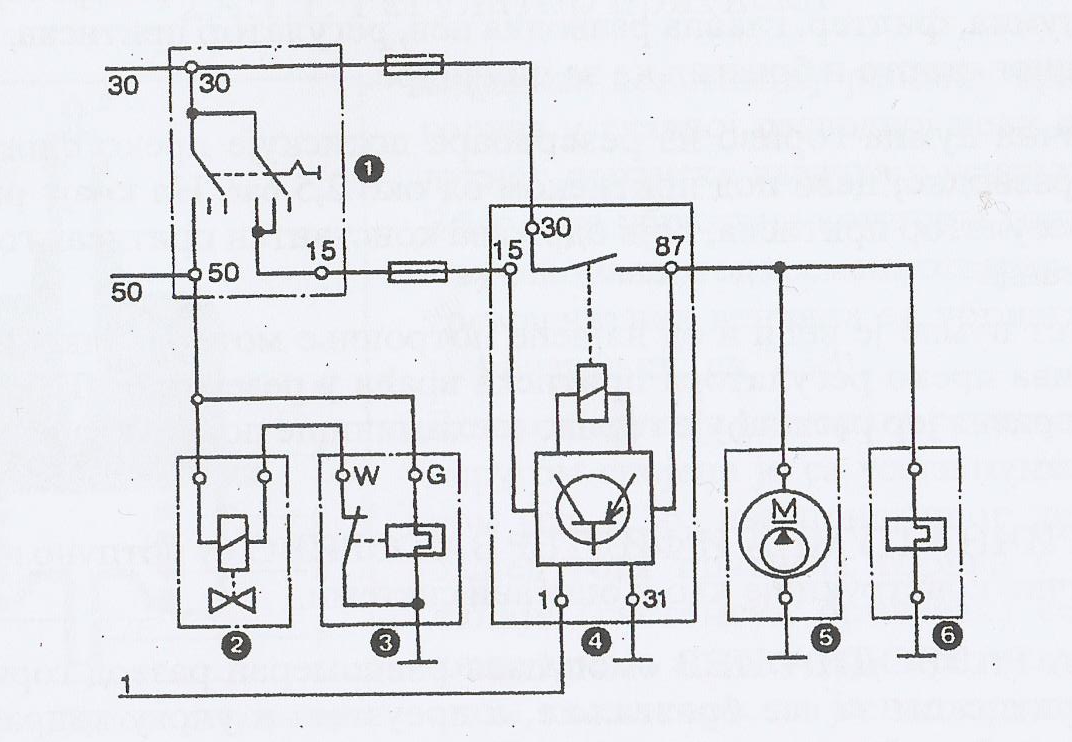
\includegraphics[width=0.9\textwidth]{slike/KEe-sis.png}
    \caption{}
    \label{fig:primer}
\end{figure}

%==================================================================
% L-JETRONIC, LH-JETRONIC, MONO-JETRONIC
% (ако користиш класу article, обриши ред са \chapter)
%==================================================================
    
\chapter{L-Jetronic систем убризгавања}

%------------------------------------------------------------------
\section{Принцип рада L-Jetronic система}
%------------------------------------------------------------------

L-Jetronic је потпуно електронски систем убризгавања. Слово L потиче од
немачке речи \textit{Luft} (ваздух), јер се количина горива одређује према
измереној количини усисаног ваздуха. Систем је настао као модификација
D-Jetronic система.

За разлику од K/KE-Jetronic-а, гориво се не убризгава непрекидно, већ у
импулсима. Свака бризгаљка је електромагнетни вентил који отвара управљачка
јединица. Притисак горива је сталан, па количина убризганог горива зависи само
од тога колико дуго је бризгаљка отворена.

Све бризгаљке убризгавају истовремено, једном по обртају коленастог вратила,
тј. два пута по радном циклусу. Сваки пут убризгају половину потребне
количине, а гориво чека испред усисног вентила.

\begin{figure}[H]
    \centering
    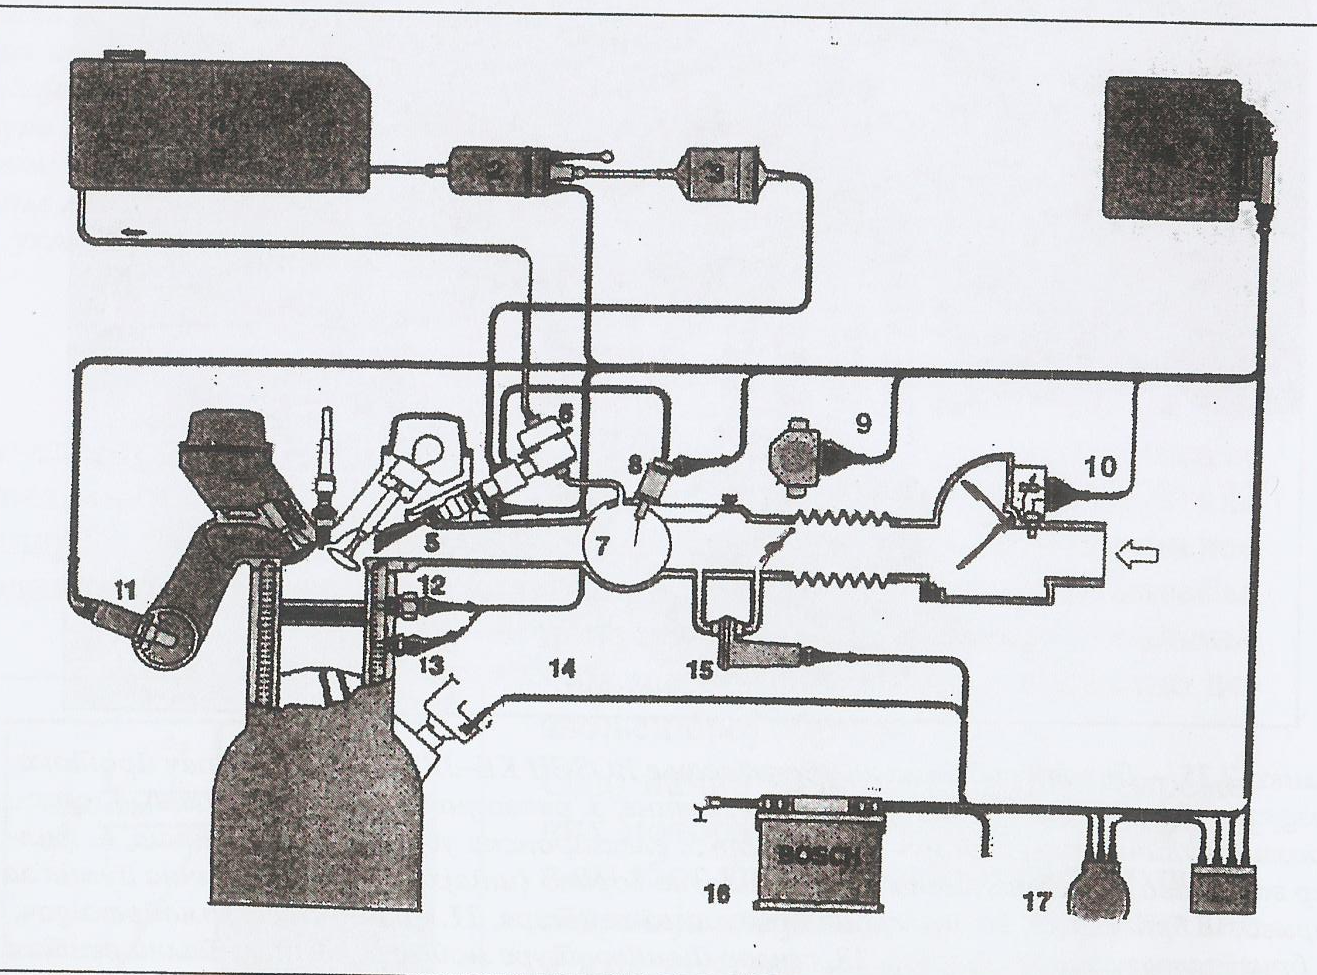
\includegraphics[width=0.7\textwidth]{slike/Le12.png}
    \caption{Шема система}
    \label{fig:primer}
\end{figure}

\begin{enumerate}
    \item[1.] Резервоар за гориво - место са бензином
    \item[2.] Електрична пумпа за гориво - потискивање горива под притиском
    \item[3.] Филтер за гориво - пречишћавање горива
    \item[4.] Електронска управљачка јединица - рачуна време убризгавања
    \item[5.] Бризгаљка - електромагнетни вентил за убризгавање
    \item[6.] Разводна цев са регулатором притиска - довод горива до бризгаљки под сталним притиском
    \item[7.] Усисни колектор - развод ваздуха до цилиндара
    \item[8.] Бризгаљка хладног старта - додатно гориво при хладном старту
    \item[9.] Прекидач пригушног лептира - сигнал празног хода и пуног оптерећења
    \item[10.] Мерач протока ваздуха (протокомер) - мерење усисаног ваздуха
    \item[11.] ЛАМБДА сонда - сензор мешавине
    \item[12.] Временски термопрекидач - укључивање бризгаљке хладног старта
    \item[13.] Сензор температуре мотора
    \item[14.] Разводник паљења - сигнал броја обртаја
    \item[15.] Биметални вентил у заобилазном воду - додатни ваздух за хладан мотор
    \item[16.] Акумулатор
    \item[17.] Контакт-кључ
\end{enumerate}

L-Jetronic систем се може поделити на три функционалне групе: 
\textbf{инсталација за напајање горивом}, \textbf{прикупљање и обрада података о мотору},
\textbf{регулација убризгавања количине горива}.

%------------------------------------------------------------------
\section{Компоненте L-Jetronic система}
%------------------------------------------------------------------

Сам по себи, L-Jetronic систем се не разликује толико пуно у односу на своје претходнике. Скоро па све компоненте 
у том систему су исте, разликују се само неке од њих, и те разлике ће бити споменуте у овом поглављу.

\subsection{Разделна цев и регулатор притиска}

Разделна цев доводи гориво до свих бризгаљки, па све имају исти притисак.

Регулатор притиска је повезан са усисном граном. Одржава сталну разлику
између притиска горива и притиска у усисној грани (око 2,5 бари). Вишак горива
враћа у резервоар. Зато иста дужина импулса увек даје исту количину горива,
без обзира на оптерећење мотора.

\begin{figure}[H]
    \centering
    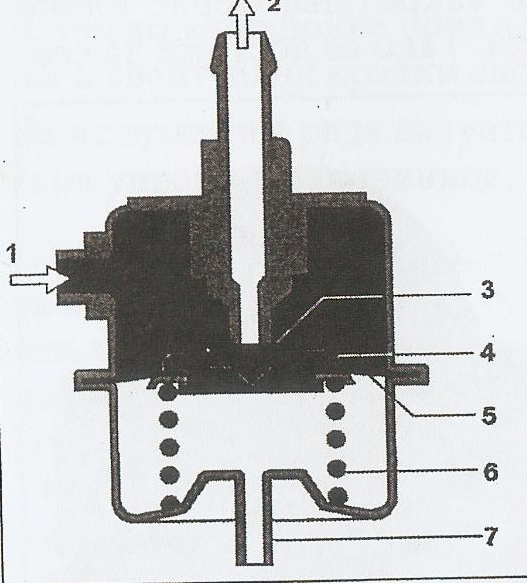
\includegraphics[width=0.4\textwidth]{slike/Le3.png}
    \caption{Rегулатор притиска}
    \label{fig:primer}
\end{figure}

\subsection{Мерење количине усисаног ваздуха}

Мерење протока ваздуха је у случају L-Jetronic система потпуно електронска,
односно преко сензора.

\begin{figure}[H]
    \centering
    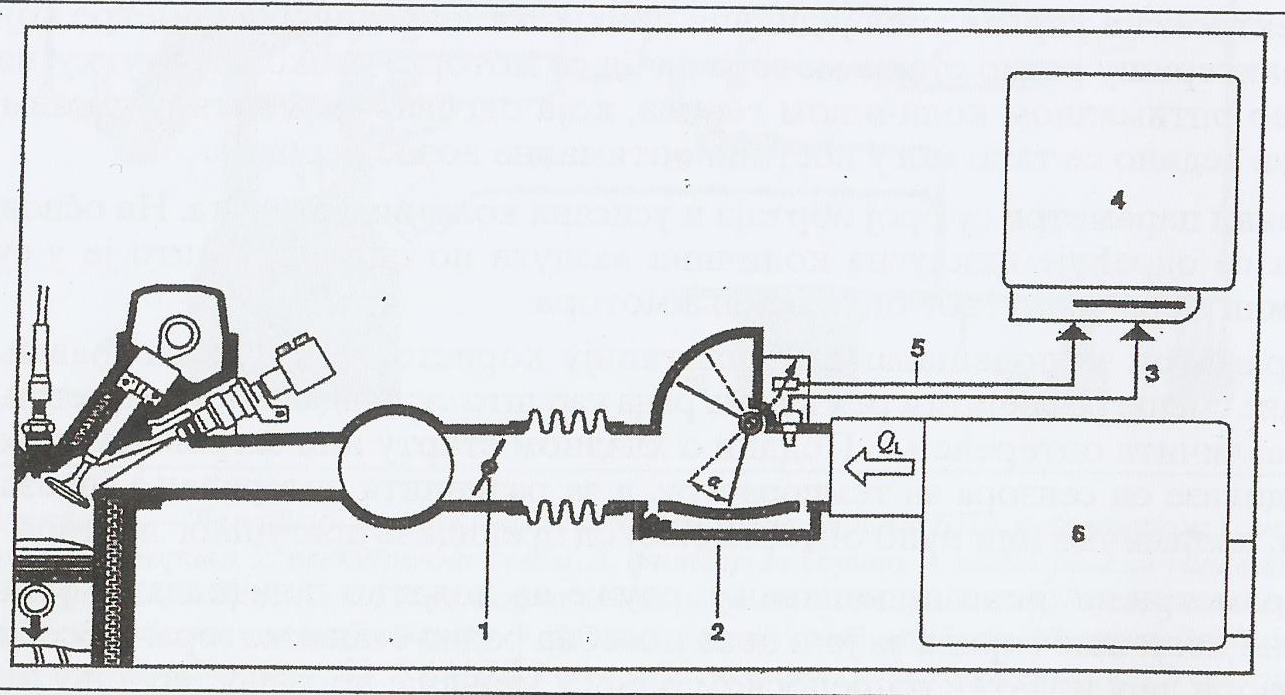
\includegraphics[width=0.4\textwidth]{slike/Le4.png}
    \caption{Мерење количине усисаног ваздуха}
    \label{fig:primer}
\end{figure}

Сензор који мери проток ваздуха назвамо \textbf{мерач протока ваздуха}
односно \textbf{протокомер}, исто као код КЕ система.

Сав усисни ваздух пролази кроз мерач. У њему је заклопка која се у струји
ваздуха закреће насупрот спиралној опрузи. Што је више ваздуха, заклопка се
више закрене. На њеној осовини је потенциометар, који управљачкој јединици
шаље напон сразмеран количини ваздуха.

Компензациона заклопка у пригушној комори смирује осцилације мерне заклопке.
Заобилазни канал са завртњем служи за подешавање састава смеше у празном ходу.

У мерачу су још:
\begin{itemize}
    \item \textbf{сензор температуре ваздуха} (Температурно зависни отпорник), јер топлији ваздух има
          мању густину, па му одговара мање горива,
    \item \textbf{контакт за пумпу}, који укључује пумпу само када ваздух
          струји, тј. када мотор ради.
\end{itemize}

\subsection{Прилагођавање радне смеше условима рада}

Прилагођавање смеше врши се помоћу компоненти: \textbf{прекидач пригушног лептира},\textbf{сензор температуре мотора}
, \textbf{ЛАМБДА регулатора}


\textbf{Прекидач пригушног лептира} остављен је на осовину пригушног лептира. Има контакт празног хода и контакт
пуног оптерећења, па управљачка јединица зна када је лептир затворен, а када
потпуно отворен.

\textbf{Сензор температуре мотора}је заправо 
емпературно зависни отпорник у облику сонде, увијен у блок мотора, са врхом у расхладној
течности. Јавља управљачкој јединици колико је мотор загрејан.

\textbf{ЛАМБДА регулација} врши се на основу сигнала од \textbf{ламбда сонде}. 
На основу одступања од идеалног случаја
ЕУЈ додатно коригује састав радне смеше, тако да средња вредност увек буде биска идеалном случају. 

\begin{figure}[H]
    \centering
    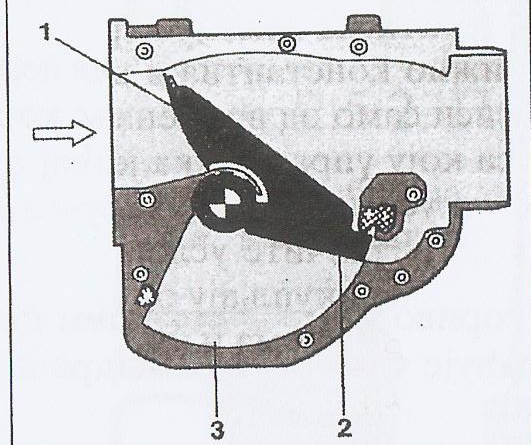
\includegraphics[width=0.4\textwidth]{slike/Le81.png}
    \caption{Ламбда регулатор}
    \label{fig:primer}
\end{figure}

\subsection{Електромагнетне бризгаљке}
 
За разлику од КЕ система, бризгаљке у L системима се контролишу електронски, на жељени такт.
Свака бризгаљка има намотај и иглу коју држи опруга. Када управљачка јединица
пусти струју кроз намотај, електромагнет подигне иглу и бризгаљка се отвори.
Када струја престане, опруга затвори иглу. Бризгаљка је отворена свега
неколико милисекунди.

\subsection{Допунски вентил за ваздух}

Налази се у заобилазном воду око пригушног лептира. Код хладног мотора
пропушта додатни ваздух, па мотор у празном ходу ради са већим бројем
обртаја. Биметална трака, загревана електричним грејачем и топлотом мотора,
постепено затвара отвор док се мотор загрева.

\subsection{Електронска управљачка јединица}

Управљачка јединица прима сигнале о:
\begin{itemize}
    \item Броју обртаја (од система паљења),
    \item Количини усисаног ваздуха,
    \item Температури ваздуха и мотора,
    \item Положају пригушног лептира,
    \item Напону акумулатора,
    \item Саставу издувних гасова (ламбда сонда, ако постоји).
\end{itemize}
На основу њих израчунава колико дуго треба држати бризгаљке отвореним.

\begin{figure}[H]
    \centering
    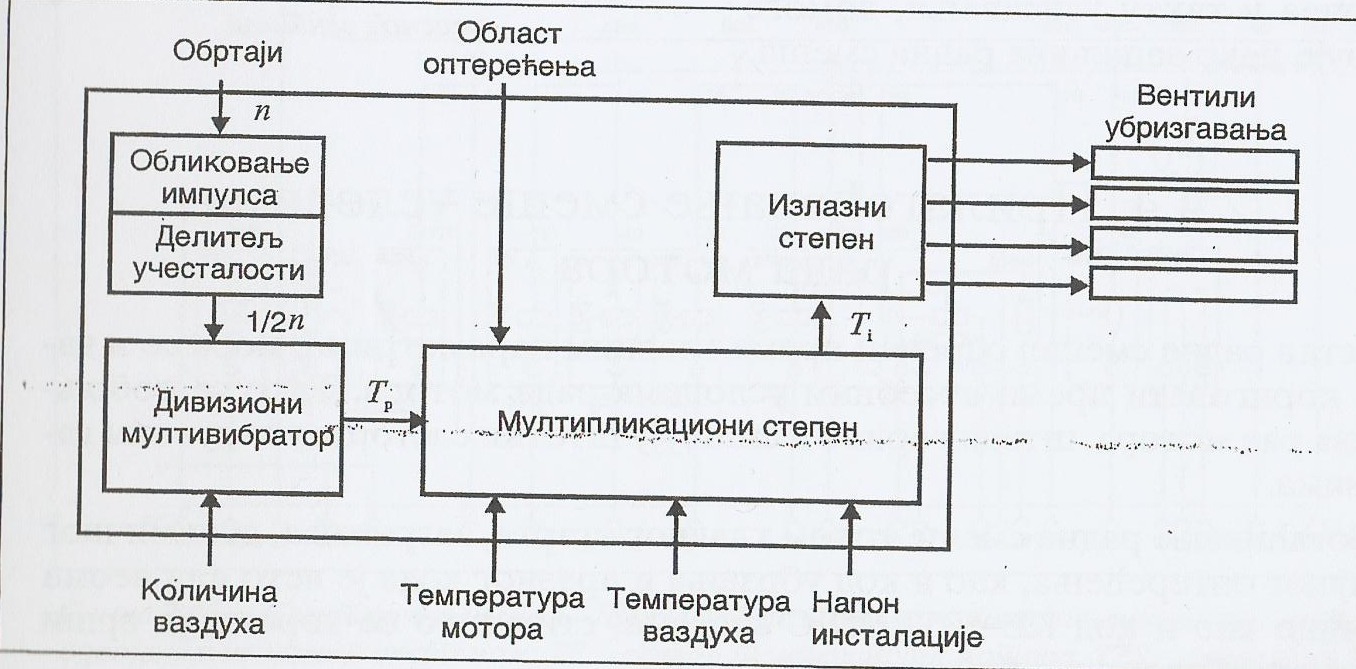
\includegraphics[width=0.5\textwidth]{slike/Le5.png}
    \caption{Електронска управљачка јединица}
    \label{fig:primer}
\end{figure}

Управљачка јединица рачуна колико времена је потребно да држи бризгаљке упаљене 
и којом учестаношћу да пали бризгаљке. Учестаност паљења бризгаљки рачуна 
на основу обртаја, температуре и притиска, а време колико ће дуго бити
упаљене бризгаљке рачуна преко следеће формуле:

\begin{equation}
    T_i = T_p + T_m + T_u
\end{equation}

Где су $T_p$ основно време импулса, $T_m$ корекција дужине импулса чије време се рачуна 
на основу температуре мотора и температуре ваздуха како би се надокнадиле евентуалне неправилности
и систему и $T_u$ је корекција напона инсталације чије време је такође последица неправилности акумулатора 
односно његове неидеалности при почетку рада мотора.

\begin{figure}[H]
    \centering
    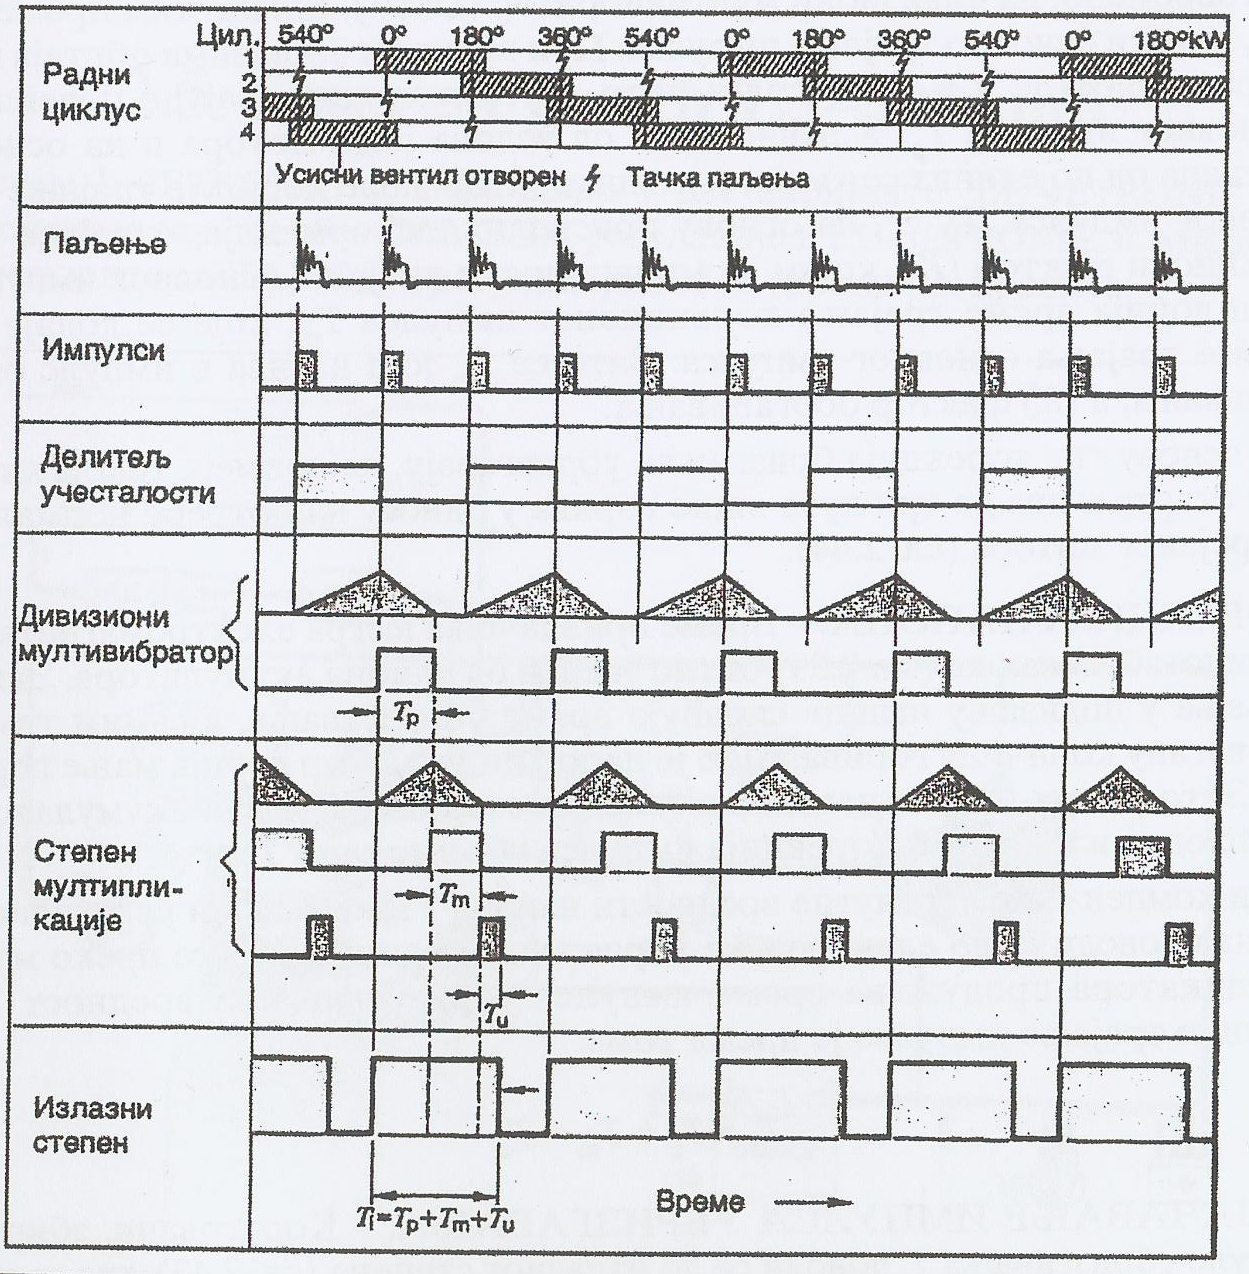
\includegraphics[width=0.5\textwidth]{slike/Le51.png}
    \caption{Рачунање тренутка убризгавања}
    \label{fig:primer}
\end{figure}

\subsection{Реле}

Реле напаја пумпу и управљачку јединицу. Пумпа ради при старту и док мотор
ради. Ако се мотор угаси, а контакт је укључен, реле искључује пумпу.

%------------------------------------------------------------------
\section{Електрична шема L-Jetronic система}
%------------------------------------------------------------------

\begin{figure}[H]
    \centering
    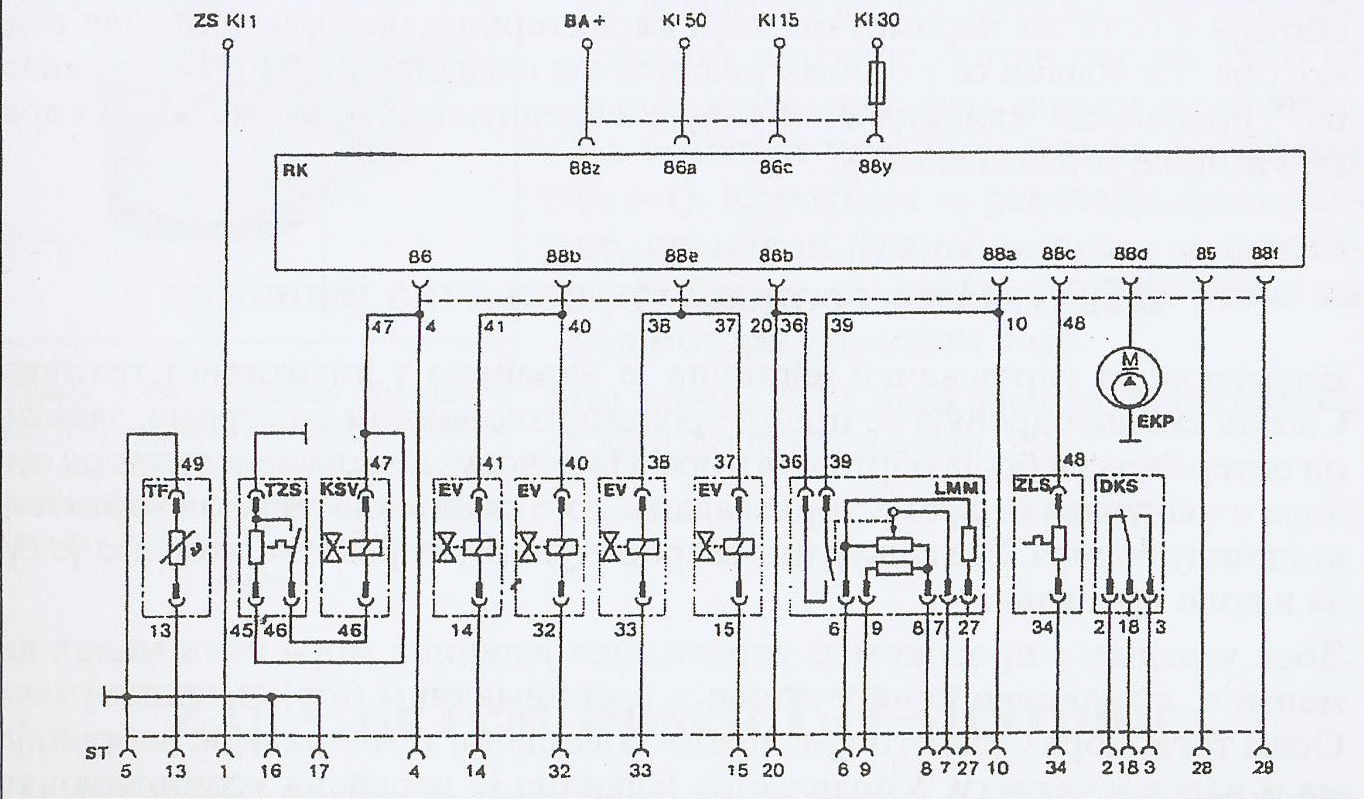
\includegraphics[width=0.6\textwidth]{slike/Le7.png}
    \caption{Електрична шема}
    \label{fig:primer}
\end{figure}

%------------------------------------------------------------------
\section{LH-Jetronic}
%------------------------------------------------------------------

\begin{figure}[H]
    \centering
    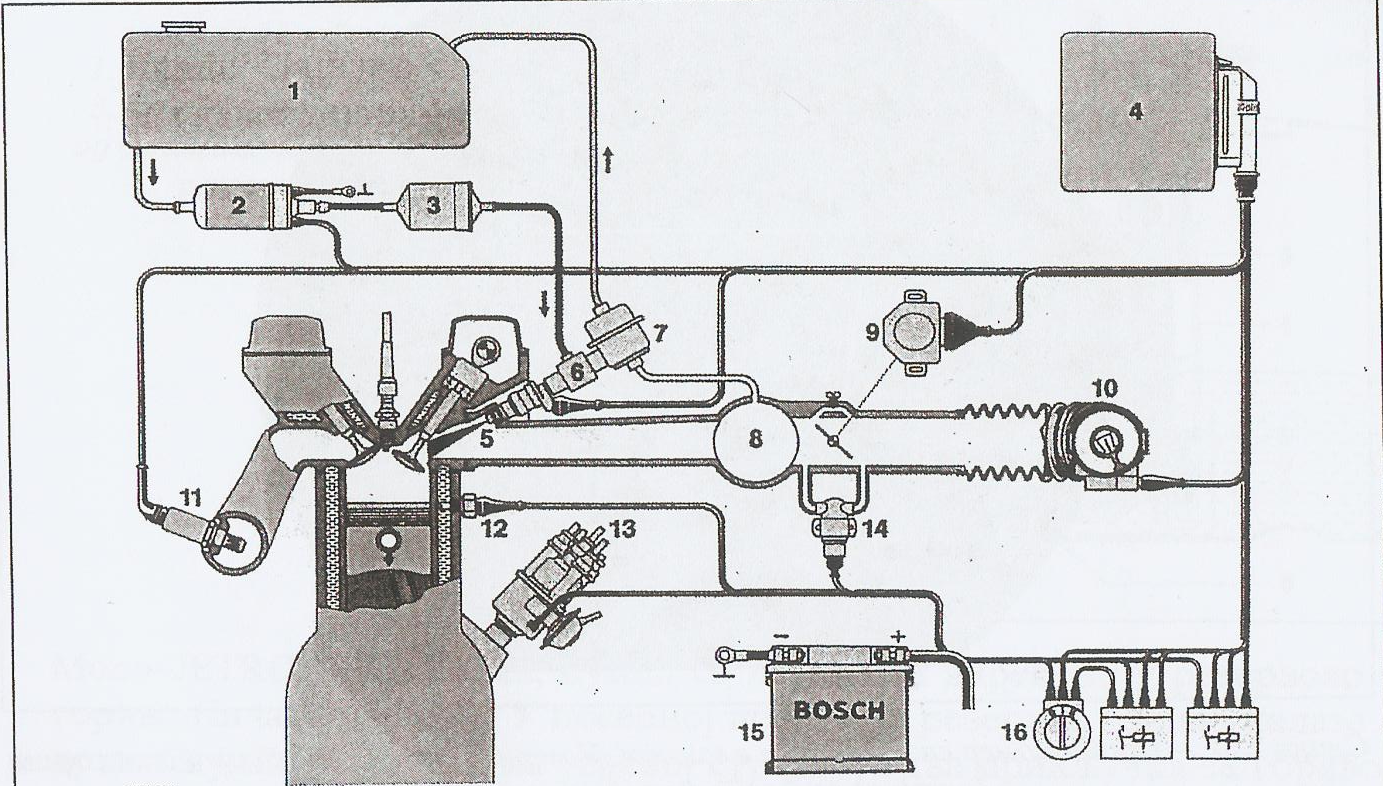
\includegraphics[width=0.8\textwidth]{slike/Le8.png}
    \caption{Шема LH-Jetronic система са компонентама}
    \label{fig:primer}
\end{figure}

\subsection{Разлика у односу на L-Jetronic}

LH-Jetronic је даљи развој L-Jetronic-а. Ознака LH потиче од \textit{Luft}
и \textit{Hitzdraht} (ваздух и врућа жица). Главна разлика је мерач: уместо
заклопке, која мери запремину ваздуха, користи се мерач који директно мери
масу ваздуха.

\subsection{Мерач масе ваздуха са врућом жицом}

У струји ваздуха разапета је танка платинска жица. Електроника је држи на
сталној температури, вишој од температуре ваздуха. Што више ваздуха протиче,
жица се више хлади и потребна је јача струја да остане загрејана. Јачина те
струје је мера масе усисаног ваздуха.

Предности у односу на заклопку:
\begin{itemize}
    \item Маса ваздуха већ обухвата његову температуру и притисак, па нису
          потребне корекције за температуру ваздуха и надморску висину,
    \item Нема покретних делова,
    \item Мањи је отпор струјању ваздуха,
    \item Мерач брже реагује на промене.
\end{itemize}

На жици се временом таложе нечистоће, које мењају мерење. Зато се после
гашења мотора жица накратко (око 1 секунду) загреје на високу температуру, па
наслаге изгоре.

\subsection{Остале новине}

Управљачка јединица је дигитална (микрорачунар), па прецизније рачуна и има
више функција. Уместо допунског вентила за ваздух користи се електрични
регулатор празног хода. Код новијих верзија обогаћивање при хладном старту
раде главне бризгаљке, без посебне бризгаљке за хладан старт. Касније је
врућа жица замењена врућим филмом, који је отпорнији.

%------------------------------------------------------------------
\section{Поређење система убризгавања}
%------------------------------------------------------------------

\begin{table}[H]
    \centering
    \small
    \begin{tabular}{p{2.6cm} p{3.4cm} p{3.4cm}}
        \toprule
                         & \textbf{K/KE-Jetronic}            & \textbf{L/LH-Jetronic}                      \\
        \midrule
        Убризгавање      & непрекидно                        & у импулсима                                \\
        Бризгаљке        & по једна за цилиндар, отвара их притисак & по једна за цилиндар, електромагнетне\\
        Мерење ваздуха   & мерна плоча                       & заклопка (L), врућа жица (LH)              \\
        Дозирање горива  & разводник (регулациони клип)      & време отварања бризгаљки                   \\
        Притисак горива  & око 5 бари                         & око 2,5-3 бари                           \\
        Електроника      & само корекције (KE)               & цело дозирање                              \\
        \bottomrule
    \end{tabular}
    \caption{Поређење система убризгавања}
    \label{tab:poredjenje}
\end{table}

\end{document}